
%%%%%%%%%%%%%%%%%%%%%%
%%%%%%%%%%%%%%%%%%%%%%
\section{Experiments and results}
%%%%%%%%%%%%%%%%%%%%%%
%%%%%%%%%%%%%%%%%%%%%%


In this section we fist analyze the average information content in a data set of experimentally annotated proteins and then evaluate performance accuracy of different function prediction methods using both topological and probabilistic metrics. Each experiment was conducted on all three categories of the Gene Ontology: Molecular Function (MFO), Biological Process (BPO), and Cellular Component (CCO) ontologies. In order to avoid cases where the information content of a term is infinite a pseudo-count of $1$ was added to each term, and the total number of proteins in the data set was incremented when calculating term frequencies.

%%%%%%%%%%%%%%%%%%%%%%
%%%%%%%%%%%%%%%%%%%%%%
\subsection{Average information content of a protein}
%%%%%%%%%%%%%%%%%%%%%%
%%%%%%%%%%%%%%%%%%%%%%

We first examined the distribution of the information content per protein for each of the three ontologies (Figure \ref{fig:rumi3}). We observe a wide range of information contents in all ontologies, reaching over 128 bits in case of BPO (which corresponds to a factor of 128 in the probability of observing particular annotation graphs). The distributions for MFO and CCO show unusual peaks for very low information contents, suggesting that a large fraction of annotation graphs in these ontologies are low quality. One such anomaly is created by the term 'binding' in MFO that is associated with 72\% of proteins. Furthermore, 41\% of proteins are annotated with its child `protein binding' as a leaf term, and 26\% are annotated with it as their sole leaf term. Such annotations, which are clearly a consequence of high-throughput experiments, present a significant difficulty in method evaluation.

%%%%%%%%%%%%%%%%%%%%%%
%%%%%%%%%%%%%%%%%%%%%%
\begin{figure*}[h!]
\begin{centering}
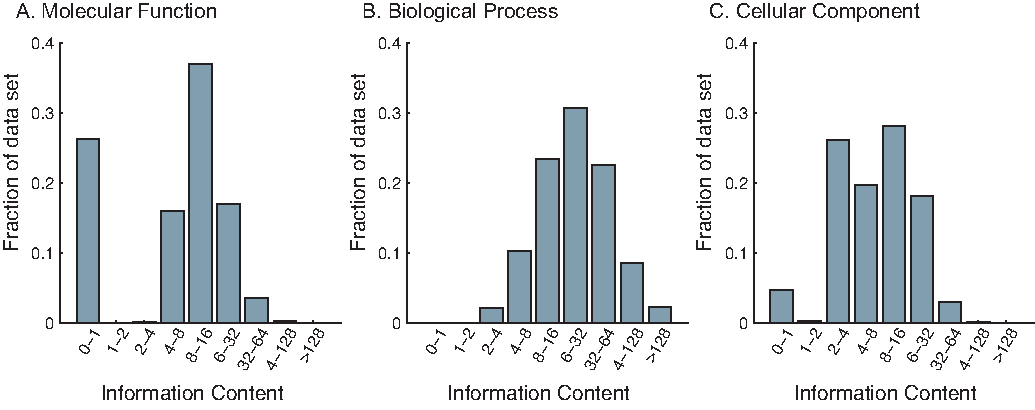
\includegraphics[width=0.85\linewidth]{Figures/rumi/Figure3}
\par\end{centering}
\caption[Distribution of information content (in bits) of protein experimental annotations]{Distribution of information content (in bits) over proteins annotated by terms for each of the three ontologies. The average information content of a protein was estimated at 10.9 (std. 10.2), 32.0 (std. 33.6), and 10.4 (std. 9.2) bits for MFO, BPO, and CCO, respectively.}
\label{fig:rumi3}
\end{figure*}
%%%%%%%%%%%%%%%%%%%%%%
%%%%%%%%%%%%%%%%%%%%%%


Previously, we showed that the distribution of leaf terms in protein annotation graphs exhibits scale-free tendencies \citep{Clark2011}. Here, we also analyzed the average number of leaf terms per protein and compared it with the information content of that protein. We estimate the average number of leaf terms to be 1.6 (std. 1.0), 3.0 (std. 3.6), and 1.6 (std. 1.0) for MFO, BPO, and CCO, respectively, and calculate Pearson correlation between the information content and the number of leaf terms for a protein (0.80, 0.92, and 0.71). Such high level of correlation suggests that proteins annotated with a small number of leaf terms are generally annotated by shallow graphs. This is particularly evident in the case of `protein binding' annotations that can be derived from yeast-2-hybrid experiments, but provide little insight into the functional aspects of these complexes when only viewed as GO annotations. We believe the wide range of information contents coupled with the fact that a large fraction of proteins were essentially uninformative, justifies the weighting proposed in this work.

%%%%%%%%%%%%%%%%%%%%%%
%%%%%%%%%%%%%%%%%%%%%%
\subsection{Two-dimensional plots}
%%%%%%%%%%%%%%%%%%%%%%
%%%%%%%%%%%%%%%%%%%%%%

In order to assess how each metric evaluated the performance of the four prediction methods we generated two-dimensional plots. Figure \ref{fig:rumi4} shows the performance of each predictor using precision/recall and ru-mi curves, as well as their weighted variants. The performance of the GO/Swiss-Prot annotation is represented as a single point because it compares two databases of experimental annotations where predictions are all binary and do not have associated scores.

%%%%%%%%%%%%%%%%%%%%%%
%%%%%%%%%%%%%%%%%%%%%%
\begin{figure*}[h!]
\begin{centering}
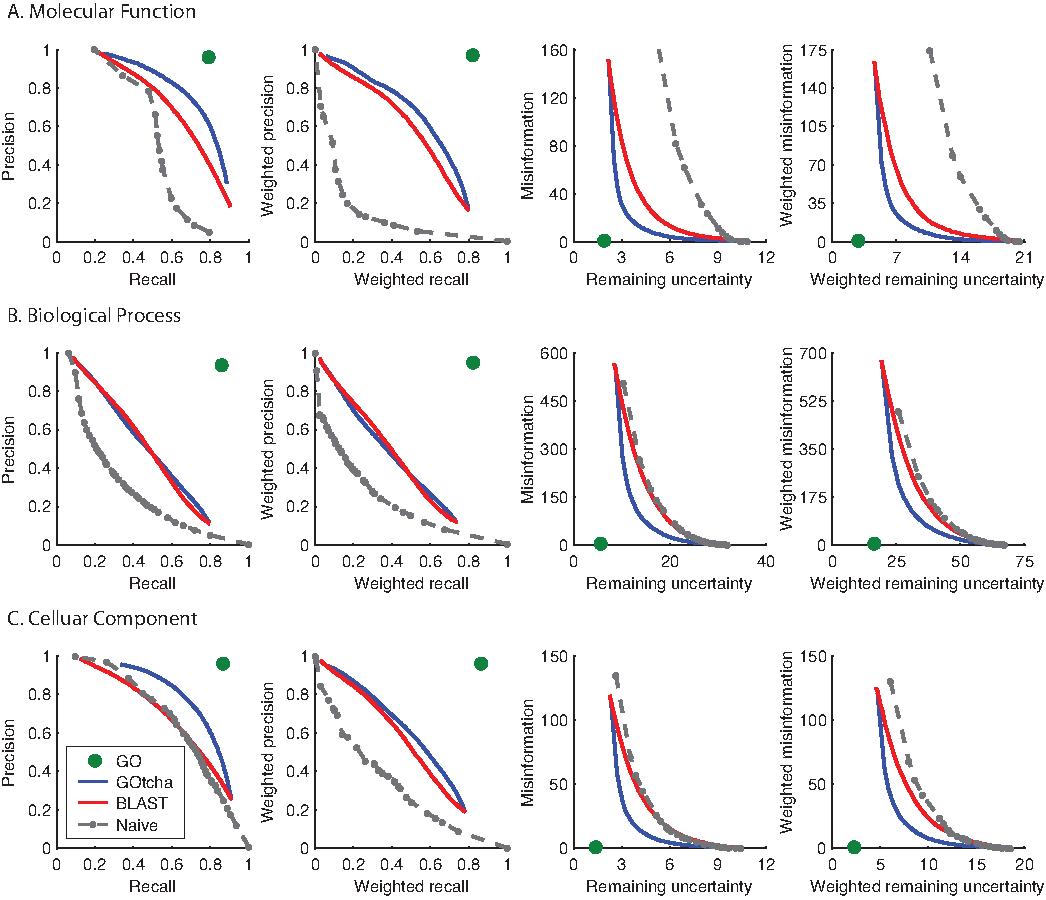
\includegraphics[width=\linewidth]{Figures/rumi/Figure4}
\end{centering}
\caption[Plots of $(pr(\tau),rc(\tau))_{\tau}$, $(wpr(\tau),wrc(\tau))_{\tau}$, $(ru(\tau),mi(\tau))_{\tau}$, and $(wru(\tau),wmi(\tau))_{\tau}$]{Two-dimensional evaluation plots. Each plot shows three prediction methods: Naive (grey, dashed), BLAST (red, solid), and GOtcha (blue, solid) constructed using cross-validation. Green point labeled GO shows the performance evaluation between two databases of experimental annotations, downloaded at the same time. The rows show the performance for different ontologies (MFO, BPO, CCO). The columns show different evaluation metrics: $(pr(\tau),rc(\tau))_{\tau}$, $(wpr(\tau),wrc(\tau))_{\tau}$, $(ru(\tau),mi(\tau))_{\tau}$, and $(wru(\tau),wmi(\tau))_{\tau}$.}
\label{fig:rumi4}
\end{figure*}
%%%%%%%%%%%%%%%%%%%%%%
%%%%%%%%%%%%%%%%%%%%%%


When looking at the precision/recall curves, we first observe an unusually high area under the curve associated with the Naive model. This is a result of a significant fraction of low information content annotations that are relatively easy to predict by simply using prior probabilities of terms as prediction values. In addition, these biases lead to a biologically unexpected result where the predictor based on the BLAST algorithm performs on par with the Naive model, e.g. $F_{\max}$(BLAST, MFO) $=0.65$ and $F_{\max}$(Naive, MFO) $=0.60$, while $F_{\max}$(BLAST, CCO) $=0.63$; $F_{\max}$(Naive, CCO) $=0.64$. The largest difference between the BLAST and Naive models was observed for BPO, which has a Gaussian-like distribution of information contents in the logarithmic scale (Figure \ref{fig:rumi3}). The second column of plots in Figure \ref{fig:rumi4} shows the weighted precision/recall curves. Here, we observe large changes in the performance accuracy, especially for the Naive model, in MFO and CCO categories, whereas the BPO category was, for the most part, not impacted. We believe that the information-theoretic weighting of precision and recall resulted in more meaningful evaluation.

In Figure \ref{fig:rumiS4}, we present more detailed results related to the ru-mi curves presented in Figure \ref{fig:rumi4}. In the top row, we show the same ru-mi curves as in the third column of Figure \ref{fig:rumi4}, with yellow dots providing information where the maximum values of semantic distance $S_2$ were reached for each method. Interestingly, because the predictors generally associate scores to all nodes in the Gene Ontology, the amount of over-prediction can be very large for low decision thresholds, which consequently results in large values of misinformation. To provide better insight into the balance between remaining uncertainty and misinformation achieved by the semantic distance $S_2$, in the bottom row we present the same curves for small values of misinformation only.

%%%%%%%%%%%%%%%%%%%%%%
%%%%%%%%%%%%%%%%%%%%%%
\begin{figure*}[h!]
\begin{centering}
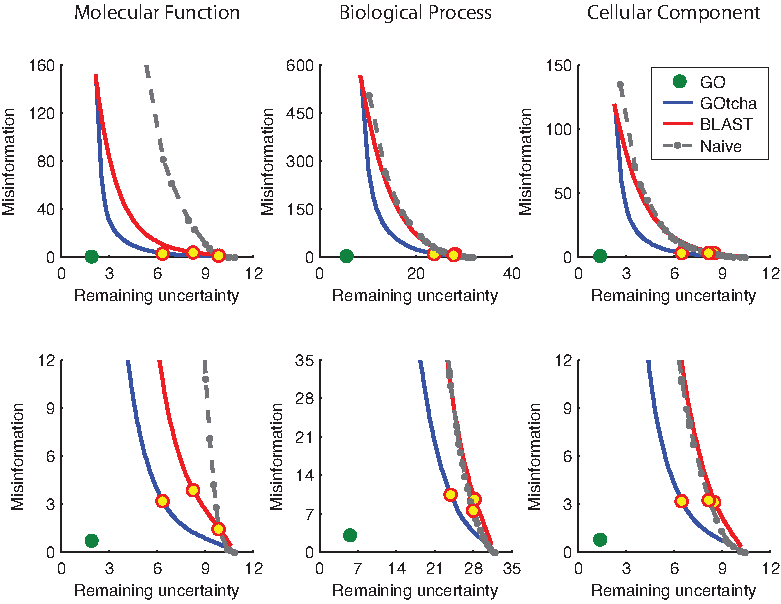
\includegraphics[width=.85\linewidth]{Figures/rumi/S4}
\end{centering}
\caption[Detailed figures showing the $ru$ and $mi$ of baseline methods]{Figures showing the remaining uncertainty and misinformation of baseline methods with yellow dots denoting values at which each method obtains its $S_{2}$ value. For better interpretation of the values at which each method achieves its $S_{2}$ value the bottom row of figures show the same plots as the top row, but with adjusted y-axis limits. }
\label{fig:rumiS4}
\end{figure*}
%%%%%%%%%%%%%%%%%%%%%%
%%%%%%%%%%%%%%%%%%%%%%


The information-theoretic measures are shown in the last two columns of Figure \ref{fig:rumi4} and in Figure \ref{fig:rumiS4}. One useful property of ru-mi plots is that they explicitly illustrate how many bits of information are yet to be revealed about a protein (on average) as a function of misinformation that is introduced by over-prediction or misannotation. In all three categories, the amount of misinformation being introduced increases rapidly; quickly obtaining a rate that is twice the amount of expected information for an average protein. We believe these plots shed new light into how much information overload a researcher can be presented with by drawing predictions at a particular threshold. Looking from right to left in each plot, we observe an elbow in each of the curves (at about 3 bits for MFO and CCO and 12 bits for BPO; Figure \ref{fig:rumi4}) after which the remaining uncertainty barely decreases, while misinformation grows out of control.

 Figure \ref{fig:rumiS1} and Figure \ref{fid:rumiS2} show results when implementing the supplemental information theoretic metrics using all-pair and max-average methods of averaging, respectively. It is important to mention that in a direct application of Resnik's similarity function, we refer to it as \emph{Lord} in Figure \ref{fig:rumiS1} (all-pair averaging) and as \emph{Resnik} in Figure \ref{fid:rumiS2} (max-average method of averaging). This is because, to the best of our knowledge, in the context of comparing functional annotations of proteins the all-pair averaging was first proposed by \citet{Lord2003}.

%%%%%%%%%%%%%%%%%%%%%%
%%%%%%%%%%%%%%%%%%%%%%
\begin{figure*}[h!]
\begin{centering}
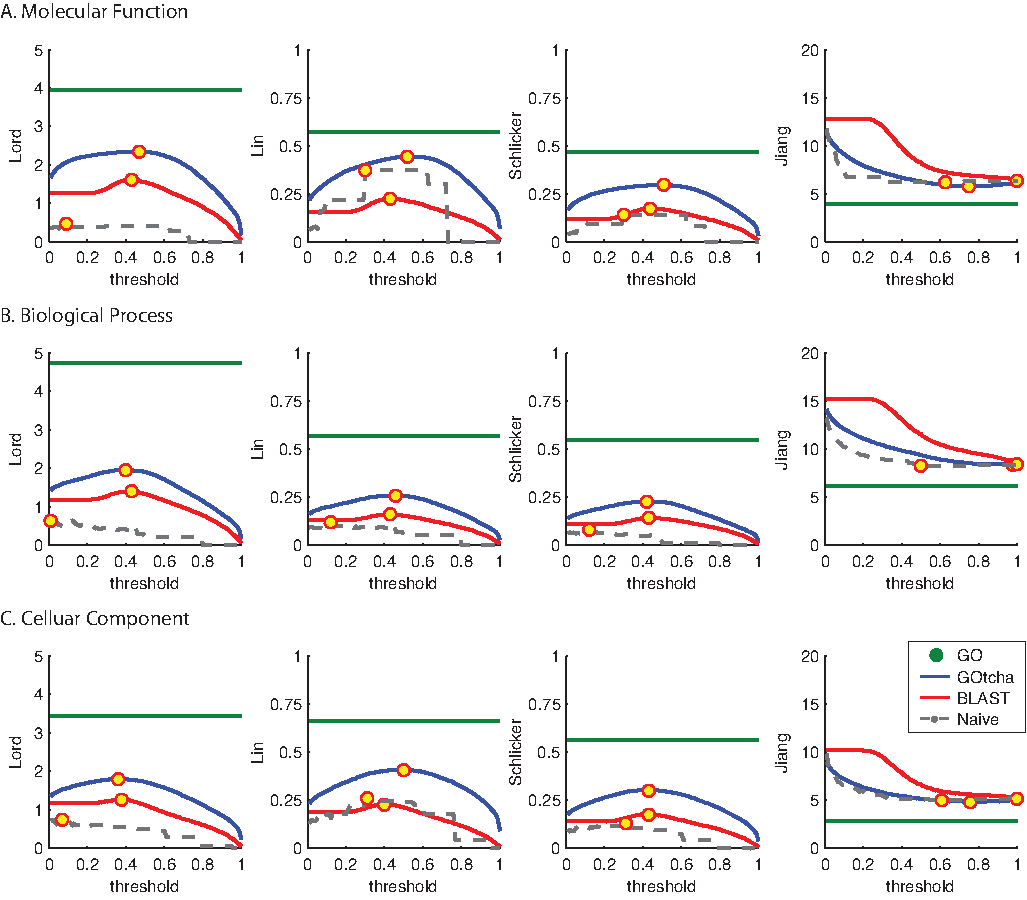
\includegraphics[width=\linewidth]{Figures/rumi/S1}
\par\end{centering}
\caption[Performance of information content-based metrics when using the all-pair method of averaging]{Two-dimensional evaluation plots of information content-based metric performances when using the all-pair method of averaging. Yellow dots denote the maximum similarity or, in the case of  \citet{Jiang1997}, the minimum distance, that each method obtains.}
\label{fig:rumiS1}
\end{figure*}
%%%%%%%%%%%%%%%%%%%%%%
%%%%%%%%%%%%%%%%%%%%%%

%%%%%%%%%%%%%%%%%%%%%%
%%%%%%%%%%%%%%%%%%%%%%
\begin{figure*}[h!]
\begin{centering}
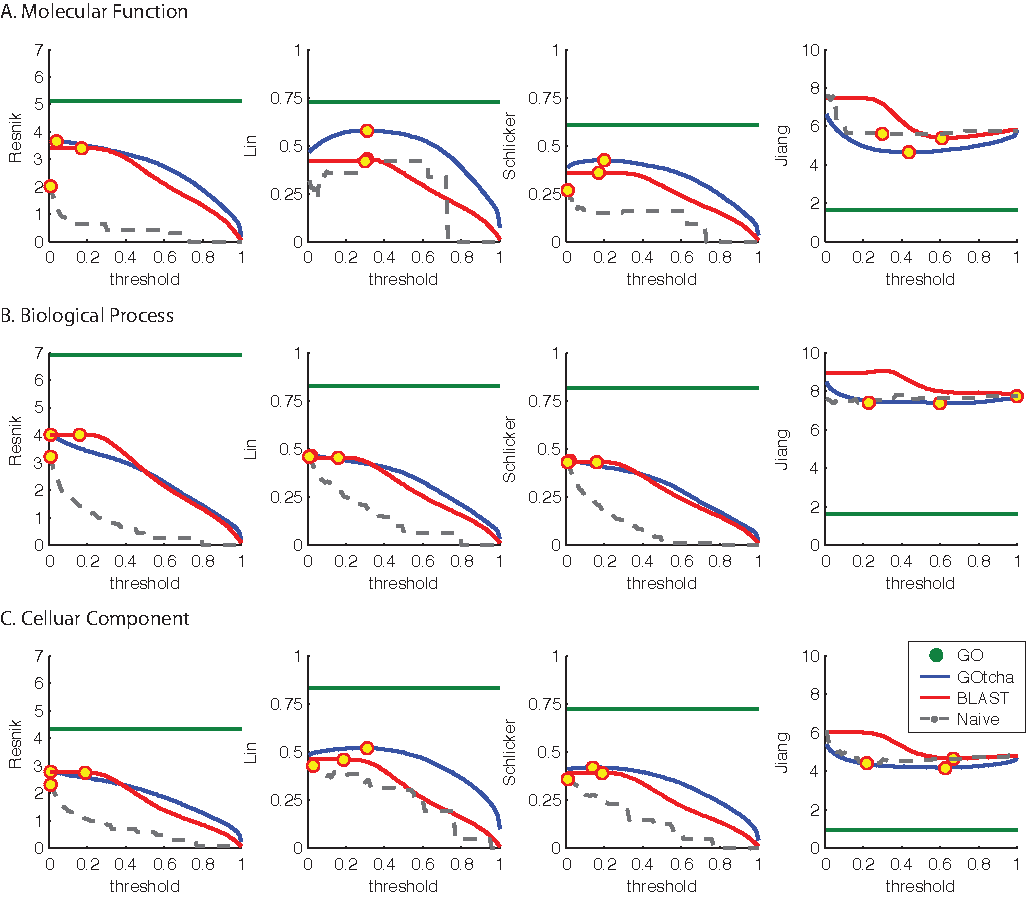
\includegraphics[width=\linewidth]{Figures/rumi/S2}
\par\end{centering}
\caption[Performance of iInformation content-based metric when using the max-average method of averaging]{Two-dimensional evaluation plots of information content-based metric performances when using the max-average method of averaging. Yellow dots denote the maximum similarity or, in the case of \citet{Jiang1997}, the minimum distance, that each method obtains.}
\label{fid:rumiS2}
\end{figure*}
%%%%%%%%%%%%%%%%%%%%%%
%%%%%%%%%%%%%%%%%%%%%%


In \Cref{fig:rumiS3} we contrast two different types of precision-recall curves. In the top row, we present the same results as in \Cref{fig:rumi3} of the main manuscript. In the bottom row, we use the max-averaging method for calculating precision-recall outlined by  \citet{Verspoor2006}. The methods provided similar results although the max-average formulation had generally larger values of $F_{\max}$ than the standard formulation of precision and recall (as defined in the main manuscript). However, these larger values of $F_{\max}$ occurred at lower decision thresholds.

%%%%%%%%%%%%%%%%%%%%%%
%%%%%%%%%%%%%%%%%%%%%%
\begin{figure*}[h!]
\begin{centering}
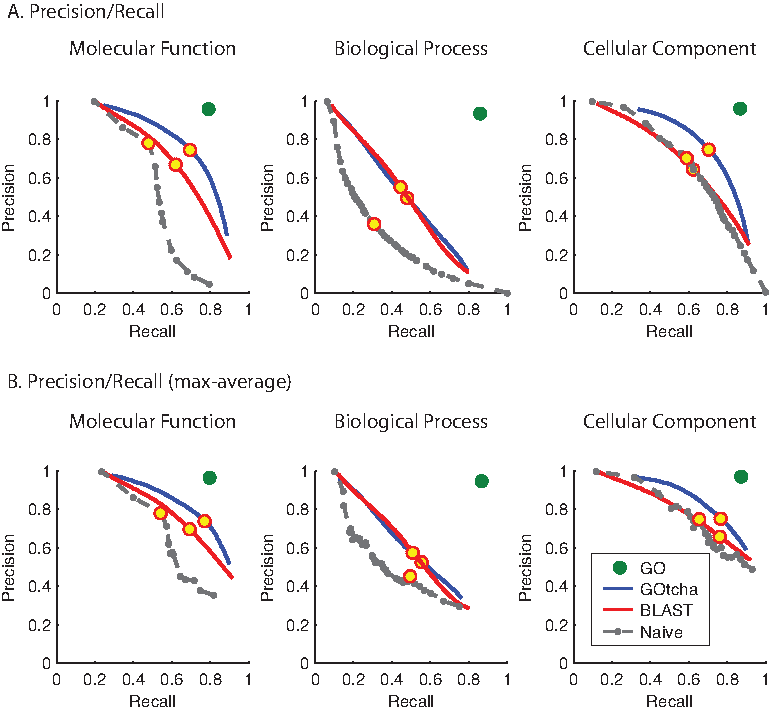
\includegraphics[width=.85\linewidth]{Figures/rumi/S3}
\par\end{centering}
\caption[Comparison of different methods of calculating precision and recall]{Plots showing results using the standard method of calculating precision and recall (top row) compared to using the max-average method of calculating precision and recall as detailed by \citet{Verspoor2006} (bottom row). Yellow dots denote the values of precision and recall at which each method obtains its $F_{\max}$ value. }
\label{fig:rumiS3}
\end{figure*}
%%%%%%%%%%%%%%%%%%%%%%
%%%%%%%%%%%%%%%%%%%%%%


%%%%%%%%%%%%%%%%%%%%%%
%%%%%%%%%%%%%%%%%%%%%%
\subsection{Comparisons of single statistics}
%%%%%%%%%%%%%%%%%%%%%%
%%%%%%%%%%%%%%%%%%%%%%

Here we analyze the ability of single measures to rank predictors and lead to useful evaluation insights. We compare the performance of semantic distance to several other methods that calculate either topological or semantic similarities. For each evaluation method, the decision threshold was varied for each of the prediction methods and the threshold providing the best performance was selected as optimal. We then analyze and discuss the performance of these metrics at those optimal thresholds.

We implemented the semantic similarity metrics of \cite{Resnik1995}, \cite{Jiang1997}, \cite{Lin1998}, and \cite{Schlicker2006}, as detailed in Section \ref{sec:rumisupmethods}. Because each of these measures is only defined for a single pair of terms in the ontology, scores between two protein annotation graphs (true graph $T$ vs. predicted graph $P$) we implemented both all pair averaging (\Cref{tab:rumi1_1,tab:rumi1_2}) and max-averaging (\Cref{tab:rumiS1}) for these metrics as detailed in Section \ref{sec:averaging}. We note that the all-pair averaging using Resnik's term similarity was implemented by \citet{Lord2003} in the context of GO annotations. In addition to these semantic measures, we also implemented the Jaccard similarity coefficient between the sets of vertices in the two annotation graphs (Section \ref{sec:rumiAddTop}). For precision/recall curves and ru-mi curves, we used $F_{\max}$ and $S_{2}$ measures as single values to obtain optimal thresholds.

Tables \ref{tab:rumi1_1}, \ref{tab:rumi1_1}, and \ref{tab:rumiS1} show the maximum similarity, or minimum distance in the case of Jiang and Conrath's and semantic distance, that each metric obtained for each of our classification models. In addition to reporting the maximum similarity we also report the decision threshold at which that value was obtained along with the associated level of remaining uncertainty and misinformation at that threshold. 

Considering \Cref{tab:rumi1_1,tab:rumi1_2} the first interesting observation is that all metrics, aside from that of Jiang and Conrath, obtain optimal thresholds that result in relatively similar levels of remaining uncertainty and misinformation for the GOtcha model. However, all metrics, aside from semantic distance and Jiang and Conrath's distance seem to favor extremely high levels of misinformation at the reported decision thresholds for the BLAST model. For MFO and CCO the semantic similarity measures of Lord \emph{et al.}, Lin and Sclicker \emph{et al.} report misinformation levels that are more than twice the information content of the average protein in that ontology for the BLAST model. In BPO those are even more extreme. We believe this is a direct consequence of the pairwise term averaging applied in these methods.

In Table \ref{tab:rumiS1}, we provide results analogous to those from Table \ref{tab:rumi1_1}, but using max-average method instead of all-pair averaging. We generally observe similar trends as before, but note that the values of BLAST thresholds used for functional transfer are even lower than when all-pair averaging was used (except for the measure by \citealt{Jiang1997}, where max-average method seems to be beneficial). 

%%%%%%%%%%%%%%%%%%%%%%
%%%%%%%%%%%%%%%%%%%%%%
\begin{table*}[t]
\caption[Performance evaluation of common information-theoretic metrics]{Performance evaluation of common information-theoretic metrics. For each measure, the decision threshold was varied across the entire range of predictions to obtain the maximum or minimum value (shown in column 1). The threshold at which each method reached the best value is shown in column 2. Columns 3 and 4 show the remaining uncertainty ($ru$) and misinformation ($mi$) calculated according to the Bayesian network. Each semantic similarity metric was calculated according to the relative frequencies of observing each term in the database. 
\label{tab:rumi1_1}}
\resizebox{\columnwidth}{!}
{\begin{tabular}{c|cccc|cccc|cccc}

\multicolumn{1}{l}{\hphantom} &\multicolumn{4}{c}{\bf Molecular Function } & \multicolumn{4}{c}{\bf Biological Process} &  \multicolumn{4}{c}{\bf Cellular Component } \\

\bf Lord & Max & Threshold & ru & mi & Max & Threshold & ru & mi & Max & Threshold & ru & mi\\
\hline
\multicolumn{1}{l|}{GOtcha}& 2.34 & 0.47 & 6.34 & 3.20 & 1.95 & 0.40 & 23.36 & 11.90 & 1.80 & 0.36 & 5.88 & 4.58 \\
\multicolumn{1}{l|}{BLAST}& 1.61 & 0.43 & 4.69 & 27.90 & 1.40 & 0.43 & 16.73 & 139.57 & 1.27 & 0.38 & 4.42 & 37.24 \\
\multicolumn{1}{l|}{Naive}& 0.46 & 0.09 & 9.56 & 4.23 & 0.63 & 0.01 & 10.35 & 504.88 & 0.75 & 0.07 & 5.81 & 16.34 \\


\multicolumn{1}{l}{\hphantom} & & & &\multicolumn{1}{c}{\hphantom} & & & & \multicolumn{1}{c}{\hphantom} & & & &\\

\bf Lin & Max & Threshold & ru & mi & Max & Threshold & ru & mi & Max & Threshold & ru & mi\\
\hline
\multicolumn{1}{l|}{GOtcha}& 0.44 & 0.52 & 6.67 & 2.67 & 0.26 & 0.46 & 24.43 & 9.40 & 0.41 & 0.50 & 6.71 & 2.76 \\
\multicolumn{1}{l|}{BLAST}& 0.22 & 0.43 & 4.69 & 27.90 & 0.16 & 0.43 & 16.73 & 139.57 & 0.23 & 0.40 & 4.78 & 30.45 \\
\multicolumn{1}{l|}{Naive}& 0.37 & 0.30 & 10.39 & 0.21 & 0.12 & 0.12 & 24.92 & 23.14 & 0.26 & 0.31 & 8.98 & 1.32 \\

\multicolumn{1}{l}{\hphantom} & & & &\multicolumn{1}{c}{\hphantom} & & & & \multicolumn{1}{c}{\hphantom} & & & &\\
%\hline
%\rowcolor{LightBlue}
\bf Schlicker & Max & Threshold & ru & mi & Max & Threshold & ru & mi & Max & Threshold & ru & mi\\
\hline
\multicolumn{1}{l|}{GOtcha}& 0.29 & 0.51 & 6.60 & 2.76 & 0.23 & 0.42 & 23.73 & 10.99 & 0.30 & 0.43 & 6.31 & 3.56 \\
\multicolumn{1}{l|}{BLAST}& 0.17 & 0.44 & 4.83 & 25.39 & 0.14 & 0.43 & 16.73 & 139.57 & 0.18 & 0.43 & 5.26 & 23.26 \\
\multicolumn{1}{l|}{Naive}& 0.14 & 0.30 & 10.39 & 0.21 & 0.08 & 0.12 & 24.92 & 23.14 & 0.13 & 0.31 & 8.98 & 1.32 \\

\multicolumn{1}{l}{\hphantom} & & & &\multicolumn{1}{c}{\hphantom} & & & & \multicolumn{1}{c}{\hphantom} & & & &\\

\bf Jiang & Min & Threshold & ru & mi & Min & Threshold & ru & mi & Min & Threshold & ru & mi\\
\hline
\multicolumn{1}{l|}{GOtcha}& 5.74 & 0.75 & 8.20 & 1.27 & 8.38 & 0.98 & 30.88 & 1.22 & 4.83 & 0.76 & 8.21 & 1.19 \\
\multicolumn{1}{l|}{BLAST}& 6.34 & 1.00 & 10.62 & 0.43 & 8.39 & 1.00 & 31.31 & 1.40 & 5.20 & 1.00 & 10.16 & 0.35 \\
\multicolumn{1}{l|}{Naive}& 6.19 & 0.63 & 10.53 & 0.13 & 8.24 & 0.50 & 31.75 & 0.07 & 5.01 & 0.61 & 10.13 & 0.08 \\


%\multicolumn{1}{l}{\hphantom} & & & &\multicolumn{1}{c}{\hphantom} & & & & \multicolumn{1}{c}{\hphantom} & & & &\\
%
%\bf Jaccard & Max & Threshold & ru & mi & Max & Threshold & ru & mi & Max & Threshold & ru & mi\\
%\hline
%\multicolumn{1}{l|}{GOtcha}& 0.57 & 0.46 & 6.29 & 3.32 & 0.31 & 0.34 & 22.24 & 15.24 & 0.56 & 0.43 & 6.31 & 3.56 \\
%\multicolumn{1}{l|}{BLAST}& 0.37 & 0.50 & 5.74 & 14.72 & 0.19 & 0.50 & 19.68 & 76.98 & 0.34 & 0.43 & 5.26 & 23.26 \\
%\multicolumn{1}{l|}{Naive}& 0.46 & 0.30 & 10.39 & 0.21 & 0.17 & 0.19 & 27.53 & 9.22 & 0.47 & 0.31 & 8.98 & 1.32 \\
%
%
%\multicolumn{1}{l}{\hphantom} & & & &\multicolumn{1}{c}{\hphantom} & & & & \multicolumn{1}{c}{\hphantom} & & & &\\
%
%$\mathbf{ F_{max} }$ & Max & Threshold & ru & mi & Max & Threshold & ru & mi & Max & Threshold & ru & mi\\
%\hline
%\multicolumn{1}{l|}{GOtcha}& 0.72 & 0.43 & 6.12 & 3.68 & 0.49 & 0.32 & 21.84 & 16.69 & 0.73 & 0.43 & 6.31 & 3.56 \\
%\multicolumn{1}{l|}{BLAST}& 0.64 & 0.48 & 5.42 & 17.89 & 0.49 & 0.50 & 19.68 & 76.98 & 0.63 & 0.45 & 5.57 & 19.42 \\
%\multicolumn{1}{l|}{Naive}& 0.60 & 0.29 & 9.87 & 1.44 & 0.33 & 0.19 & 27.53 & 9.22 & 0.64 & 0.33 & 9.22 & 0.80 \\
%
%
%\multicolumn{1}{l}{\hphantom} & & & &\multicolumn{1}{c}{\hphantom} & & & & \multicolumn{1}{c}{\hphantom} & & & &\\
%
%$\mathbf{S_{2}}$  & Min & Threshold & ru & mi & Max & Threshold & ru & mi & Max & Threshold & ru & mi\\
%\hline
%\multicolumn{1}{l|}{GOtcha}& 7.11 & 0.47 & 6.34 & 3.20 & 26.14 & 0.43 & 23.91 & 10.56 & 7.23 & 0.46 & 6.48 & 3.21 \\
%\multicolumn{1}{l|}{BLAST}& 9.13 & 0.77 & 8.25 & 3.90 & 29.89 & 0.88 & 28.28 & 9.69 & 9.08 & 0.78 & 8.51 & 3.15 \\
%\multicolumn{1}{l|}{Naive}& 9.98 & 0.10 & 9.72 & 2.80 & 29.00 & 0.22 & 27.67 & 8.72 & 8.79 & 0.21 & 7.71 & 4.95 \\

%\end{tabular}}{Values marked in bold are interesting .  Might want to say more, but really probably don't need to here.}
\end{tabular}}{}
\end{table*}
%%%%%%%%%%%%%%%%%%%%%%
%%%%%%%%%%%%%%%%%%%%%%



\begin{table*}[t]
\caption[Performance evaluation of topological metrics and $S_{2}$]{Performance evaluation of topological metrics and $S_{2}$. For each measure, the decision threshold was varied across the entire range of predictions to obtain the maximum or minimum value (shown in column 1). The threshold at which each method reached the best value is shown in column 2. Columns 3 and 4 show the remaining uncertainty ($ru$) and misinformation ($mi$) calculated according to the Bayesian network. Each semantic similarity metric was calculated according to the relative frequencies of observing each term in the database. 
\label{tab:rumi1_2}}
\resizebox{\columnwidth}{!}
{\begin{tabular}{c|cccc|cccc|cccc}

\multicolumn{1}{l}{\hphantom} &\multicolumn{4}{c}{\bf Molecular Function } & \multicolumn{4}{c}{\bf Biological Process} &  \multicolumn{4}{c}{\bf Cellular Component } \\

\bf Jaccard & Max & Threshold & ru & mi & Max & Threshold & ru & mi & Max & Threshold & ru & mi\\
\hline
\multicolumn{1}{l|}{GOtcha}& 0.57 & 0.46 & 6.29 & 3.32 & 0.31 & 0.34 & 22.24 & 15.24 & 0.56 & 0.43 & 6.31 & 3.56 \\
\multicolumn{1}{l|}{BLAST}& 0.37 & 0.50 & 5.74 & 14.72 & 0.19 & 0.50 & 19.68 & 76.98 & 0.34 & 0.43 & 5.26 & 23.26 \\
\multicolumn{1}{l|}{Naive}& 0.46 & 0.30 & 10.39 & 0.21 & 0.17 & 0.19 & 27.53 & 9.22 & 0.47 & 0.31 & 8.98 & 1.32 \\


\multicolumn{1}{l}{\hphantom} & & & &\multicolumn{1}{c}{\hphantom} & & & & \multicolumn{1}{c}{\hphantom} & & & &\\

$\mathbf{ F_{max} }$ & Max & Threshold & ru & mi & Max & Threshold & ru & mi & Max & Threshold & ru & mi\\
\hline
\multicolumn{1}{l|}{GOtcha}& 0.72 & 0.43 & 6.12 & 3.68 & 0.49 & 0.32 & 21.84 & 16.69 & 0.73 & 0.43 & 6.31 & 3.56 \\
\multicolumn{1}{l|}{BLAST}& 0.64 & 0.48 & 5.42 & 17.89 & 0.49 & 0.50 & 19.68 & 76.98 & 0.63 & 0.45 & 5.57 & 19.42 \\
\multicolumn{1}{l|}{Naive}& 0.60 & 0.29 & 9.87 & 1.44 & 0.33 & 0.19 & 27.53 & 9.22 & 0.64 & 0.33 & 9.22 & 0.80 \\


\multicolumn{1}{l}{\hphantom} & & & &\multicolumn{1}{c}{\hphantom} & & & & \multicolumn{1}{c}{\hphantom} & & & &\\

$\mathbf{S_{2}}$  & Min & Threshold & ru & mi & Min & Threshold & ru & mi & Min & Threshold & ru & mi\\
\hline
\multicolumn{1}{l|}{GOtcha}& 7.11 & 0.47 & 6.34 & 3.20 & 26.14 & 0.43 & 23.91 & 10.56 & 7.23 & 0.46 & 6.48 & 3.21 \\
\multicolumn{1}{l|}{BLAST}& 9.13 & 0.77 & 8.25 & 3.90 & 29.89 & 0.88 & 28.28 & 9.69 & 9.08 & 0.78 & 8.51 & 3.15 \\
\multicolumn{1}{l|}{Naive}& 9.98 & 0.10 & 9.72 & 2.80 & 29.00 & 0.22 & 27.67 & 8.72 & 8.79 & 0.21 & 7.71 & 4.95 \\

%\end{tabular}}{Values marked in bold are interesting .  Might want to say more, but really probably don't need to here.}
\end{tabular}}{}
\end{table*}
%%%%%%%%%%%%%%%%%%%%%%
%%%%%%%%%%%%%%%%%%%%%%




It is particularly interesting to analyze the optimal thresholds obtained for the BLAST model. These thresholds can be interpreted as the level of sequence identity above which each metric reports  functional transfer can be made. For example, because their optimal BLAST thresholds are relatively low, the levels of misinformation provided by the similarities of Lord \emph{et al.}, Lin, and Schlicker \emph{et al.} are rather large in both tables. $F_{\max}$ and Jaccard approaches also report low threshold values for all ontologies, while Jiang and Conrath's distance selects the optimal threshold at an overly restrictive 100\% sequence identity. We believe that the semantic distance $S_2$ provides more reasonable values for functional transfer, finding an optimal distance at 77\%, 88\% and 78\% for MFO, BPO, and CCO, respectively.

We believe that, generally, all-pair averaging provides better results regarding functional similarity than does max-average.  This is predominantly based on the even lower optimal thresholds obtained for the BLAST model in Table \ref{tab:rumiS1}.

%%%%%%%%%%%%%%%%%%%%%%
%%%%%%%%%%%%%%%%%%%%%%
\begin{table*}[h!]
\caption[Performance evaluation of metrics using max-averaging]{Performance of information-theoretic methods when calculating performance as the average of maximum similarity (or distance) between each true and predicted term as described in Section \ref{sec:averaging}. $F_{\max}$ values were calculated using precision and recall as detailed by  \citet{Verspoor2006}. The decision threshold was varied across the entire range of predictions to obtain the maximum or minimum value (shown in column 1) for each method. The threshold at which each method reached the best value is shown in column 2. Columns 3 and 4 show the remaining uncertainty and misinformation calculated according to the Bayesian network.
\label{tab:rumiS1}}
\resizebox{\columnwidth}{!}
{\begin{tabular}{c|cccc|cccc|cccc}

\multicolumn{1}{l}{\hphantom} &\multicolumn{4}{c}{\bf Molecular Function } & \multicolumn{4}{c}{\bf Biological Process} &  \multicolumn{4}{c}{\bf Cellular Component } \\


\bf Resnik & Max & Threshold & ru & mi & Max & Threshold & ru & mi & Max & Threshold & ru & mi\\
\hline
\multicolumn{1}{l|}{GOtcha}& 3.65 & 0.04 & 2.96 & 32.17 & 4.02 & 0.01 & 10.19 & 273.90 & 2.80 & 0.01 & 2.70 & 59.02 \\
\multicolumn{1}{l|}{BLAST}& 3.41 & 0.17 & 2.17 & 151.77 & 4.03 & 0.16 & 8.48 & 566.88 & 2.77 & 0.19 & 2.26 & 119.34 \\
\multicolumn{1}{l|}{Naive}& 2.02 & 0.01 & 5.07 & 177.91 & 3.22 & 0.01 & 10.35 & 504.88 & 2.32 & 0.01 & 2.65 & 135.04 \\


\multicolumn{1}{l}{\hphantom} & & & &\multicolumn{1}{c}{\hphantom} & & & & \multicolumn{1}{c}{\hphantom} & & & &\\

\bf Lin & Max & Threshold & ru & mi & Max & Threshold & ru & mi & Max & Threshold & ru & mi\\
\hline
\multicolumn{1}{l|}{GOtcha}& 0.58 & 0.31 & 5.32 & 5.86 & 0.46 & 0.02 & 11.10 & 192.89 & 0.52 & 0.31 & 5.55 & 5.58 \\
\multicolumn{1}{l|}{BLAST}& 0.43 & 0.31 & 2.90 & 90.72 & 0.45 & 0.16 & 8.48 & 566.88 & 0.46 & 0.19 & 2.26 & 119.34 \\
\multicolumn{1}{l|}{Naive}& 0.42 & 0.30 & 10.39 & 0.21 & 0.46 & 0.01 & 10.35 & 504.88 & 0.43 & 0.03 & 3.90 & 56.83 \\


\multicolumn{1}{l}{\hphantom} & & & &\multicolumn{1}{c}{\hphantom} & & & & \multicolumn{1}{c}{\hphantom} & & & &\\

\bf Jiang & Min & Threshold & ru & mi & Min & Threshold & ru & mi & Min & Threshold & ru & mi\\
\hline
\multicolumn{1}{l|}{GOtcha}& 4.65 & 0.44 & 6.18 & 3.56 & 7.39 & 0.60 & 26.65 & 5.30 & 4.19 & 0.63 & 7.45 & 1.80 \\
\multicolumn{1}{l|}{BLAST}& 5.38 & 0.61 & 6.97 & 7.58 & 7.75 & 1.00 & 31.31 & 1.40 & 4.67 & 0.67 & 7.84 & 5.13 \\
\multicolumn{1}{l|}{Naive}& 5.61 & 0.30 & 10.39 & 0.21 & 7.41 & 0.23 & 27.73 & 8.49 & 4.45 & 0.22 & 8.17 & 3.25 \\


\multicolumn{1}{l}{\hphantom} & & & &\multicolumn{1}{c}{\hphantom} & & & & \multicolumn{1}{c}{\hphantom} & & & &\\

\bf Schlicker & Max & Threshold & ru & mi & Max & Threshold & ru & mi & Max & Threshold & ru & mi\\
\hline
\multicolumn{1}{l|}{GOtcha}& 0.42 & 0.20 & 4.56 & 9.32 & 0.44 & 0.02 & 11.10 & 192.89 & 0.42 & 0.14 & 4.29 & 12.76 \\
\multicolumn{1}{l|}{BLAST}& 0.36 & 0.17 & 2.17 & 151.77 & 0.43 & 0.16 & 8.48 & 566.88 & 0.39 & 0.19 & 2.26 & 119.34 \\
\multicolumn{1}{l|}{Naive}& 0.27 & 0.01 & 5.07 & 177.91 & 0.43 & 0.01 & 10.35 & 504.88 & 0.36 & 0.01 & 2.65 & 135.04 \\

\multicolumn{1}{l}{\hphantom} & & & &\multicolumn{1}{c}{\hphantom} & & & & \multicolumn{1}{c}{\hphantom} & & & &\\

$\mathbf{ F_{max} }$ & Max & Threshold & ru & mi & Max & Threshold & ru & mi & Max & Threshold & ru & mi\\
\hline
\multicolumn{1}{l|}{GOtcha}& 0.76 & 0.33 & 5.45 & 5.41 & 0.54 & 0.23 & 19.79 & 26.04 & 0.76 & 0.31 & 5.55 & 5.58 \\
\multicolumn{1}{l|}{BLAST}& 0.70 & 0.44 & 4.83 & 25.39 & 0.54 & 0.46 & 18.06 & 108.73 & 0.71 & 0.37 & 4.23 & 41.17 \\
\multicolumn{1}{l|}{Naive}& 0.64 & 0.29 & 9.87 & 1.44 & 0.47 & 0.07 & 22.06 & 51.55 & 0.70 & 0.20 & 7.23 & 6.75 \\


\end{tabular}}{}
\end{table*}
%%%%%%%%%%%%%%%%%%%%%%
%%%%%%%%%%%%%%%%%%%%%%


%\vskip -0.5in

%\begin{table}
%\processtable{BLAST threshold that produces the optimal score for each of the metrics. BLAST score provides sequence identity above which the metrics favor transfer of function from each protein in the database to the target protein. 
%\label{Tab:02}}
%{\begin{tabular}{l|cccccc|c}

%\multicolumn{1}{l|}{\hphantom} & \bf Lord & \bf Lin & \bf Schlicker & \bf Jiang  & \bf Jaccard & $%\mathbf{ F_{max} }$ & $\mathbf{S_{2}}$ \\
%\hline
%\bf MFO & 0.43 & 0.43 & 0.44 & 1 & 0.5 & 0.48 & 0.77\\
%\bf BPO & 0.43 & 0.43 & 0.43 & 1 & 0.5 & 0.5 & 0.88\\
%\bf CCO  & 0.38 & 0.4 & 0.43 & 1 & 0.43 & 0.45 & 0.78\\

%\end{tabular}}{Values marked in bold are interesting .  Might want to say more, but really probably don't need to here.}
%\end{tabular}}{}
%\end{table}



